
\documentclass{beamer}
\usepackage[10pt]{extsizes} 
\usepackage[T2A]{fontenc}
\usepackage[utf8]{inputenc}
\usepackage[english,russian]{babel}
%\usepackage{pscyr}
\usepackage{hyperref}
\usepackage{setspace}
\usepackage{amsmath,amssymb,amsfonts,amsthm,secdot}

\usetheme{focus} % Use the Focus theme supplied with the template
% Add option [numbering=none] to disable the footer progress bar
% Add option [numbering=fullbar] to show the footer progress bar as always full with a slide count

% Uncomment to enable the ice-blue theme
%\definecolor{main}{RGB}{92, 138, 168}
%\definecolor{background}{RGB}{240, 247, 255}

%------------------------------------------------

\usepackage{booktabs} % Required for better table rules

%----------------------------------------------------------------------------------------
%	 TITLE SLIDE
%----------------------------------------------------------------------------------------

\title{Тема: \\ Методы трассировки лучей }

\subtitle{Методы Монте-Карло}

\author{Михайлин Д.А.}



\date{02.05.2019}

%------------------------------------------------

\begin{document}

%------------------------------------------------

\begin{frame}
	\maketitle 
\end{frame}

%----------------------------------------------------------------------------------------
%	 SECTION 1
%----------------------------------------------------------------------------------------

\section{Основные понятия.} % Section title slide, unnumbered

%------------------------------------------------

\begin{frame}{Поток}
	\begin{columns}
		\column{0.5\textwidth}
			Поток излучения обозначается - $\Phi$(Flux). 
		
		\column{0.5\textwidth}
			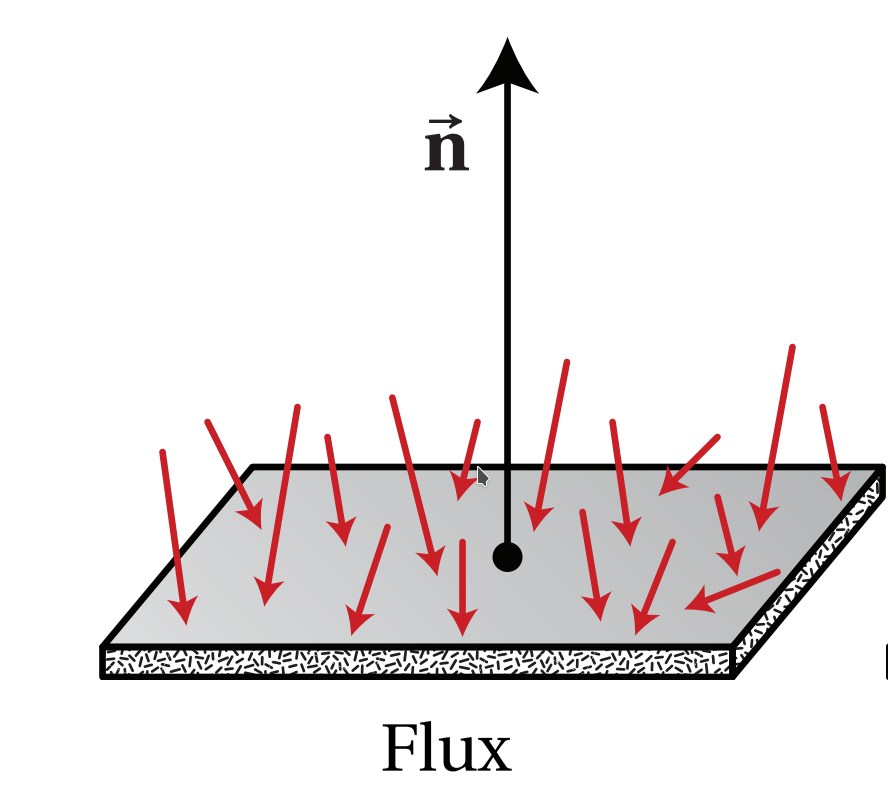
\includegraphics[width=\linewidth]{Flux.png}
	\end{columns}
\end{frame}

\begin{frame}{Интенсивность излучения}
	\begin{columns}
		\column{0.5\textwidth}
			Интенсивность излучения обозначается - E(Irradiance). $E = \frac{d\Phi(x)}{dS(x)}$
		
		\column{0.5\textwidth}
			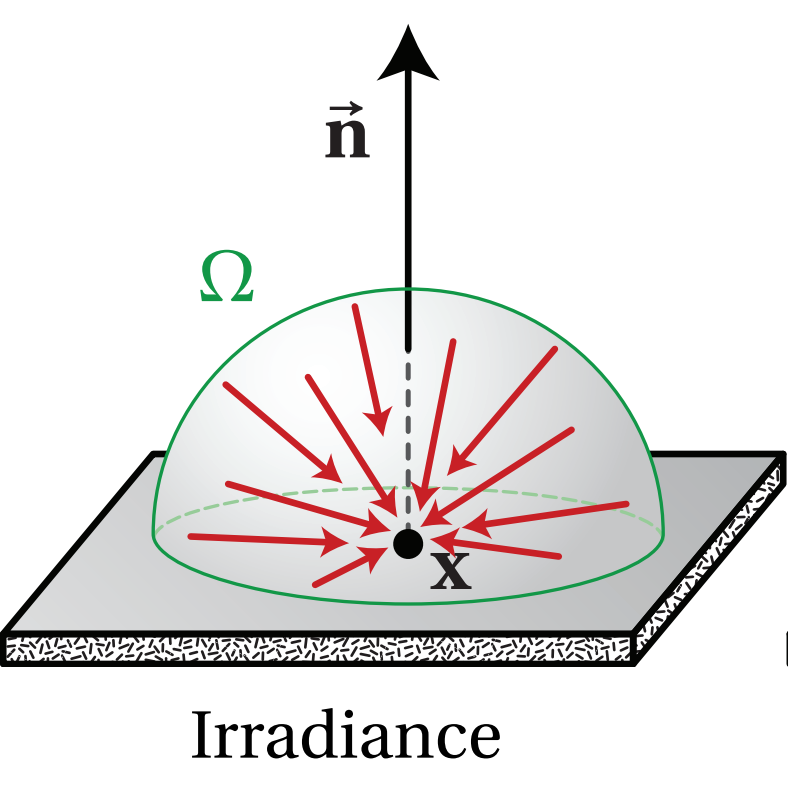
\includegraphics[width=\linewidth]{Irradiance.png}
	\end{columns}
\end{frame}
\begin{frame}{Cветимость}
	\begin{columns}
		\column{0.5\textwidth}
			Светимость обозначается - L(Radiance).\\ $L(x, \omega) = \frac{d^2\Phi(x)}{d\omega(x)dA^{\perp}(x)}$ \\ Можно переписать это уравнение в виде: \\$L(x, \omega) = \frac{d^2\Phi(x)}{d\omega(x)dA(x)(\omega, n)} = \frac{d^2\Phi(x)}{d\omega^{\perp}(x)dA(x)}$ 
		
		\column{0.5\textwidth}
			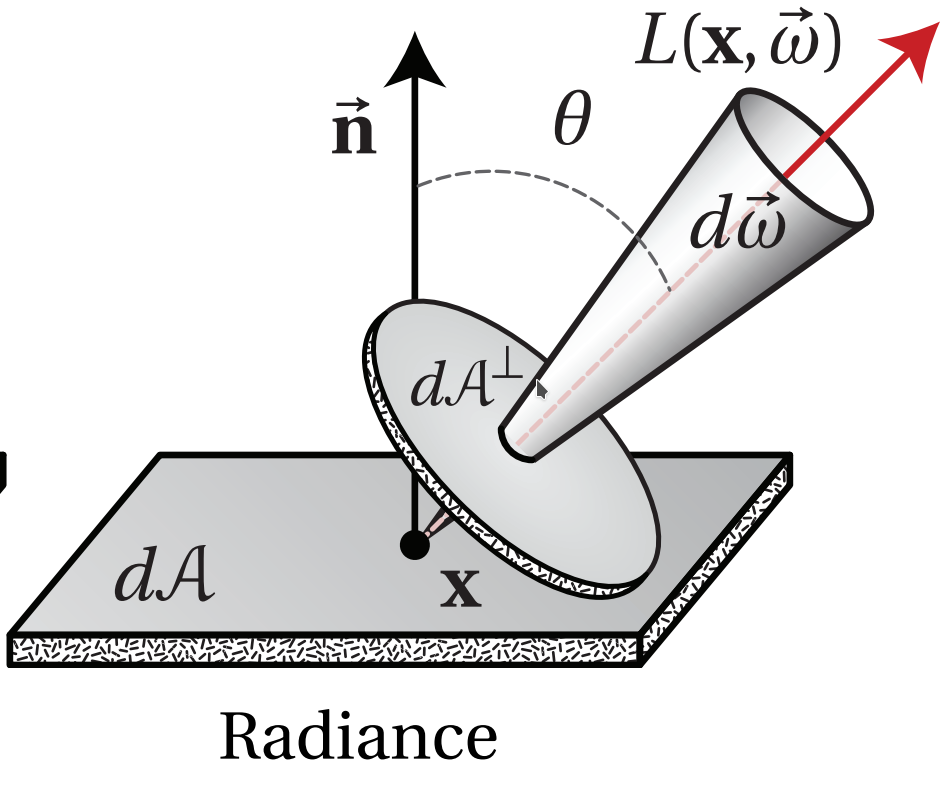
\includegraphics[width=\linewidth]{Radiance.png}
	\end{columns}
\end{frame}

\begin{frame}{Cвязь между этими величинами:}
	$L(x, \omega) = \frac{d^2\Phi(x)}{d\omega(x)dA^{\perp}(x)}$;\\ $L(x, \omega)d\omega(x)dA^{\perp}(x) = d^2\Phi(x)$;\\ $\Phi(x) = \int_A \int_{\Omega} L(x, \omega)d\omega(x)dA^{\perp}(x)$ = $\int_A \int_{\Omega} L(x, \omega)(\omega, n)d\omega(x)dA(x)$ \\ Получили выражение для потока через светимость. \\ 
	Также можем выразить интенсивность излучения через светимость. \\
	$E(x) = \int_{\Omega}L(x,\omega)(\omega, n)d\omega = \int_{\Omega}L(x, \omega)d\omega^{\perp}$
	
\end{frame}

\begin{frame}{BRDF}
	Bidirectional reflectance distribution function. Эта функция описывает насколько "ярко" выглядит поверхность с направления $\omega$.\\
	$f_r(x, \omega_1\rightarrow\omega) = \frac{dL(x\rightarrow\omega)}{dE(x\leftarrow\omega_1)} = \frac{dL(x\rightarrow\omega)}{L(x\leftarrow\omega_1)(n,\omega_1)d\omega_1}$
	
\end{frame}

\begin{frame}{Основное уравнение рендеринга.}
	Bidirectional reflectance distribution function. Эта функция описывает насколько "ярко" выглядит поверхность с направления $\omega$.\\
	$f_r(x, \omega_1\rightarrow\omega) = \frac{dL(x\rightarrow\omega)}{dE(x\leftarrow\omega_1)} = \frac{dL(x\rightarrow\omega)}{L(x\leftarrow\omega_1)(n,\omega_1)d\omega_1}$
	
\end{frame}
%------------------------------------------------

\begin{frame}[plain]{Plain Slide}
	This is a slide with the plain style and it is numbered.
\end{frame}

%------------------------------------------------

\begin{frame}[t]
	This slide has an empty title and is aligned to top.
\end{frame}

%------------------------------------------------

\begin{frame}[noframenumbering]{No Slide Numbering}
	This slide is not numbered and is citing reference \cite{knuth74}.
\end{frame}

%------------------------------------------------

\begin{frame}{Typesetting and Math}
	The packages \texttt{inputenc} and \texttt{FiraSans}\footnote{\url{https://fonts.google.com/specimen/Fira+Sans}}\textsuperscript{,}\footnote{\url{http://mozilla.github.io/Fira/}} are used to properly set the main fonts.
	\vfill
	This theme provides styling commands to typeset \emph{emphasized}, \alert{alerted}, \textbf{bold}, \textcolor{example}{example text}, \dots
	\vfill
	\texttt{FiraSans} also provides support for mathematical symbols:
	\begin{equation*}
		e^{i\pi} + 1 = 0.
	\end{equation*}
\end{frame}

%----------------------------------------------------------------------------------------
%	 SECTION 2
%----------------------------------------------------------------------------------------

\section{Section 2}

%------------------------------------------------

\begin{frame}{Blocks}
	These blocks are part of 1 slide, to be displayed consecutively.
	\begin{block}{Block}
		Text.
	\end{block}
	\pause % Automatically creates a new "page" split between the above and above + below
	\begin{alertblock}{Alert block}
		Alert \alert{text}.
	\end{alertblock}
	\pause % Automatically creates a new "page" split between the above and above + below
	\begin{exampleblock}{Example block}
		Example \textcolor{example}{text}.
	\end{exampleblock}
\end{frame}

%------------------------------------------------

\begin{frame}{Columns}
	\begin{columns}
		\column{0.5\textwidth}
			This text appears in the left column and wraps neatly with a margin between columns.
		
		\column{0.5\textwidth}
			
\includegraphics[width=\linewidth]{Images/placeholder.jpg}
	\end{columns}
\end{frame}

%------------------------------------------------

\begin{frame}{Lists}
	\begin{columns}[T, onlytextwidth] % T for top align, onlytextwidth to suppress the margin between columns
		\column{0.33\textwidth}
			Items:
			\begin{itemize}
				\item Item 1
				\begin{itemize}
					\item Subitem 1.1
					\item Subitem 1.2
				\end{itemize}
				\item Item 2
				\item Item 3
			\end{itemize}
		
		\column{0.33\textwidth}
			Enumerations:
			\begin{enumerate}
				\item First
				\item Second
				\begin{enumerate}
					\item Sub-first
					\item Sub-second
				\end{enumerate}
				\item Third
			\end{enumerate}
		
		\column{0.33\textwidth}
			Descriptions:
			\begin{description}
				\item[First] Yes.
				\item[Second] No.
			\end{description}
	\end{columns}
\end{frame}

%------------------------------------------------

\begin{frame}{Table}
	\begin{table}
		\centering % Centre the table on the slide
		\begin{tabular}{l c}
			\toprule
			Discipline & Avg. Salary \\
			\toprule
			\textbf{Engineering} & \textbf{\$66,521} \\
			Computer Sciences & \$60,005\\
			Mathematics and Sciences & \$61,867\\
			Business & \$56,720\\
			Humanities \& Social Sciences & \$56,669\\
			Agriculture and Natural Resources & \$53,565\\
			Communications & \$51,448\\
			\midrule
			\textbf{Average for All Disciplines} & \textbf{\$58,114}\\
			\bottomrule
		\end{tabular}
	\caption{Table caption}
	\end{table}
\end{frame}

%------------------------------------------------

\begin{frame}[focus]
	Thanks for using \textbf{Focus}!
\end{frame}

%----------------------------------------------------------------------------------------
%	 CLOSING/SUPPLEMENTARY SLIDES
%----------------------------------------------------------------------------------------

\appendix

\begin{frame}{References}
	\nocite{*} % Display all references regardless of if they were cited
	\bibliography{example.bib}
	\bibliographystyle{plain}
\end{frame}

%------------------------------------------------

\begin{frame}{Backup Slide}
	This is a backup slide, useful to include additional materials to answer questions from the audience.
	\vfill
	The package \texttt{appendixnumberbeamer} is used to refrain from numbering appendix slides.
\end{frame}

%----------------------------------------------------------------------------------------

\end{document}
